\subsection{Sensitivity analysis}
\label{sec:netzero_evaluation}

We carry out the experiments based on a real data center, called Net-zero Energy Data Centers (NEDC) invented by HP \cite{arlitt2012towards}. 
In NEDC, the total local generation (i.e. PV and GE generations) is greater than the total power consumption. NEDC have an additional constraint
$$\sum_{t=1}^{T}\sum_{r=1}^{R}c_{r}(y,t) + \sum_{t=1}^{T}\sum_{s=1}^{S}c_{s}(y,t) \geq \sum_{t=1}^{T}P(y,t), \quad \forall y,$$
where the left hand side and the right hand side are the total power generation and the total power consumption in year $y$, respectively.

We focus on studying the impacts of supply and demand factors on the data centers during the first year. The supply factors include electricity price, and gas price. The demand factors include shape of interactive workload and ratio of flexible workload. Besides the capacities and expenditures of the data center, we study the payback period, which is the number of years for the data center to recoup the investment in the infrastructure costs of PV and GE instead of using only the electricity grid. The shorter payback period is, the more financial benefit the proposed framework provides.

\subsubsection{Impacts of supply factors}

\hideit{
\begin{figure}[!ht]
%matlab: TCO_grid_electricity_0115.m
\vspace{-0.1cm}
\begin{center}
	\subfigure[Capacity]{{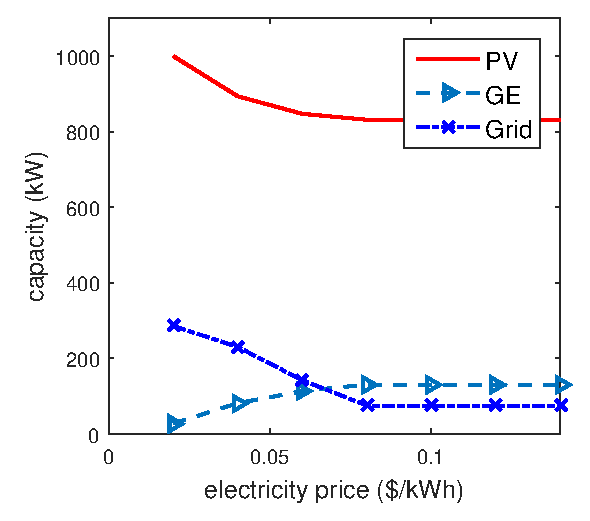
\includegraphics[width=0.32\columnwidth]{figs/capacity_electricity}}
		\label{f.capacity_electricity}}
	\subfigure[Payback period]{{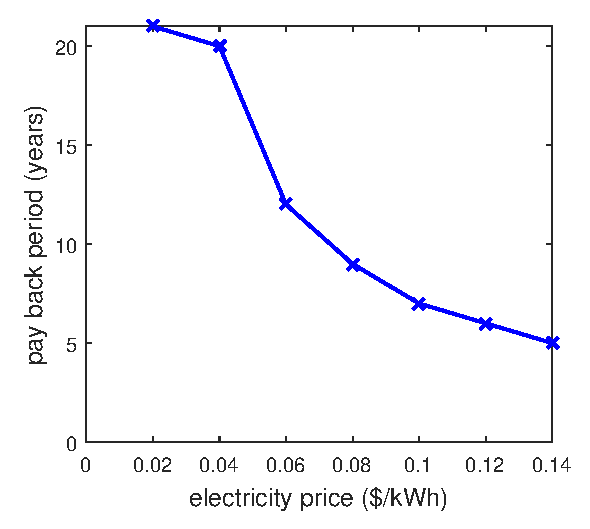
\includegraphics[width=0.32\columnwidth]{figs/payback_electricity}}
		\label{f.payback_electricity}}
	\caption{Impacts of electricity prices. As the electricity price increases, the capacity of GE is increased to compensate for the PV generation during nighttime. Interestingly, it results in reducing the capacity of PV.}
	\label{f.electricity}
\end{center}
\vspace{-0.3cm}
\end{figure}
}

\emph{Electricity price}. Figure~\ref{f.electricity} presents the impacts of electricity prices on the proposed framework. Figure~\ref{f.capacity_electricity} shows that the data center uses more GE generation and less grid power when the electricity price increases. However, the data center surprisingly keeps reducing the capacity of PV. It is because the data center starts to use more GE to provide power during nighttime and replace PV during daytime. It is because the costs of GE are relatively lower than the infrastructure of PV as PV is not fully utilized around its peak generation. In addition, when the grid power becomes more expensive, the payback period sharply decreases as in Figure \ref{f.payback_electricity}. Hence, the NEDC can significantly gain financial benefits when the electricity prices are high.
\hideit{
\begin{figure}[!ht]
%	\vspace{-0.3cm}
\begin{center}
	\subfigure[Capacity]{{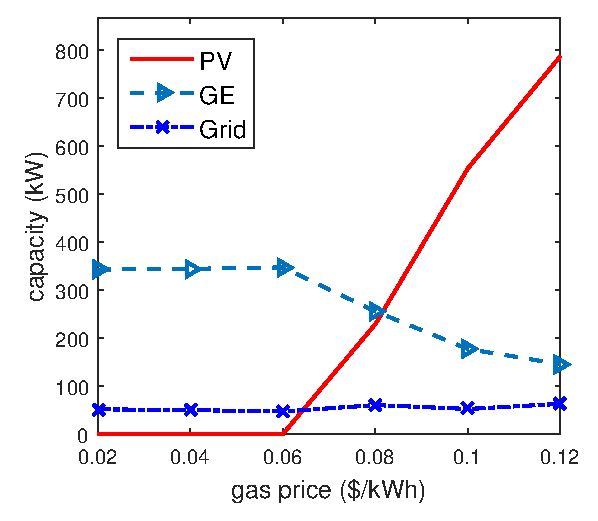
\includegraphics[width=0.32\columnwidth]{figs/capacity_gas}}
		\label{f.capacity_gas}}
	%        \subfigure[Cost]{{\includegraphics[width=0.48\columnwidth]{figs/cost_gas}}
	%            \label{f.cost_gas}}
	\subfigure[Payback period]{{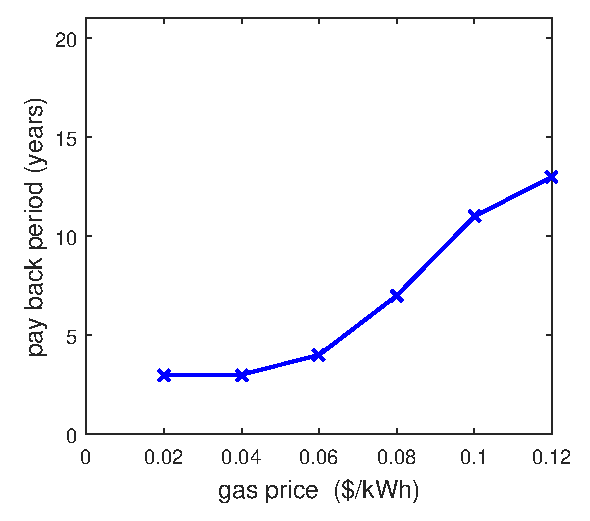
\includegraphics[width=0.32\columnwidth]{figs/payback_gas}}
		\label{f.payback_gas}}
 \vspace{-0.3cm}
	\caption{Impacts of gas prices. As the gas prices increase, the capacity of PV increases quickly because the data center cannot import too much electricity grid.}
	\label{f.gas}
\end{center}
\vspace{-0.3cm}
\end{figure}
}
\emph{Gas price.} Figure~\ref{f.gas} shows the impacts of gas prices on capacities and payback periods. In Figure \ref{f.capacity_gas}, the data center should use the GE generation at low gas prices, but it switches using PV when the gas price is more expensive. Especially, there is the sharp increase of PV capacity when the gas price is greater than $0.06$. Due to the non-dispatchability of solar energy, the data center needs the large capacity of PV generation to compensate for the reduction of GE generation. As the gas price increases, the payback period goes up as in Figure \ref{f.payback_gas} because the data center needs more PV.

\begin{figure}[!ht]
	%matlab: TCO_grid_payback_pv.m or TCO_grid_surface.m
	\begin{center}
		\subfigure[Capacity]{{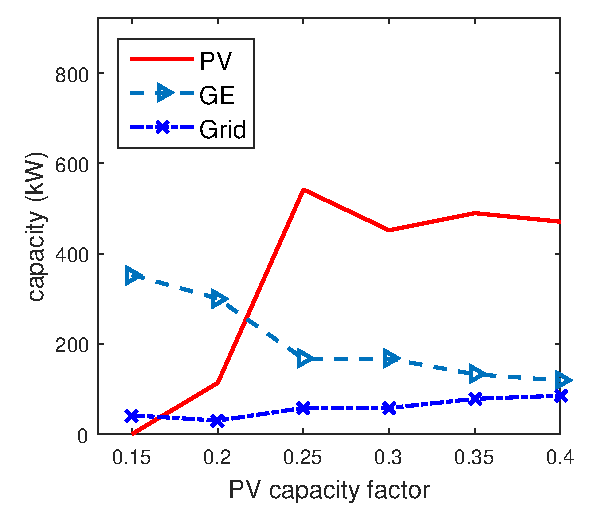
\includegraphics[width=0.32\columnwidth]{figs/capacity_PV}}
			\label{f.capacity_PV}}
		%        \subfigure[Cost]{{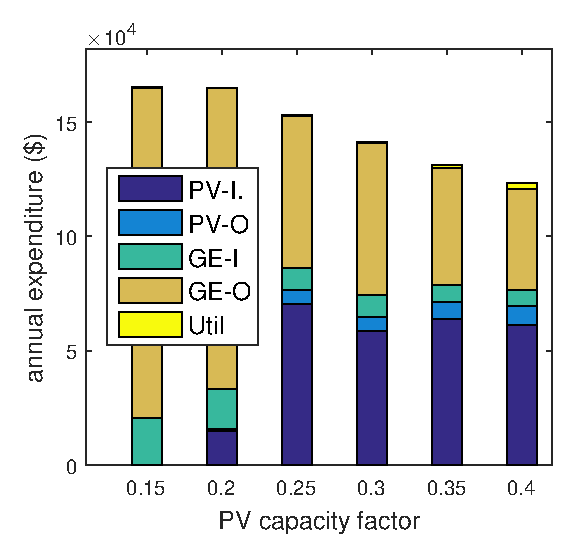
\includegraphics[width=0.48\columnwidth]{figs/cost_PV}}
		%            \label{f.cost_PV}}
		\subfigure[Payback period]{{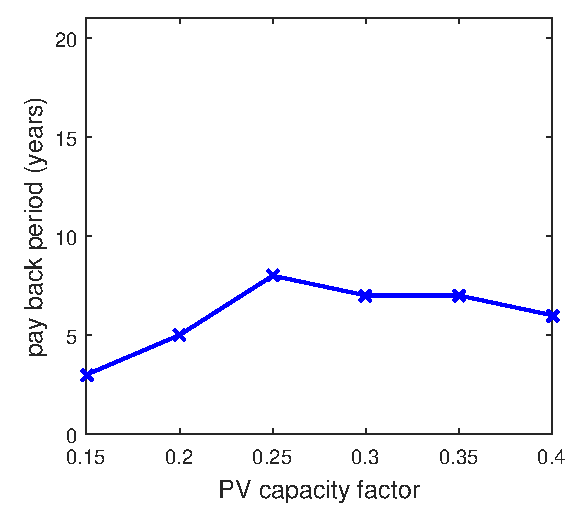
\includegraphics[width=0.32\columnwidth]{figs/payback_PV}}
			\label{f.payback_PV}}
		\caption{Impact of different PV capacity factors. The curves of PV are very interesting which goes up and down because the high capacity factors have strong impact on the capital cost and operational cost of PV.}
		\label{f.PV}
	\end{center}
\end{figure}

\new{
	\emph{PV capacity factor.} To understand how PV capacity factors affect on the proposed framework, we run the experiments with various capacity factors of PV.
	Recall the capacity factor is the average power generated, divided by the rated peak power. Figure {\ref{f.PV}} shows the dependence of the capacities and payback periods of the data center on PV capacity factors. The capacity of PV increases and then varies at high capacity factors. The capacity factor of PV array varies due to diverse reasons, such as geographical conditions. When PV has enough efficiency, i.e. capacity factor varies from 0.15 to 0.25, the data center starts to use PV. At a very high capacity factor (0.25-0.4), it is not necessary to increase the PV capacity because even the lower capacity with high capacity factors can still provide enough generation.}

\textbf{\textit{Key insight}}: The capacities of PV, GE, and peak power of grid power consumption adapt to the variety of supply factors accordingly. (i) The impacts of electricity prices and gas prices show the trade-offs between PV and GE. (ii) Under the increase of electricity price, the capacity of PV unexpectedly goes down together with the peak grid power.	(iii) Under a certain gas price, the data center does not provision PV generation but only use GE and grid power instead.\delete{(iii) The impacts of PV capacity factors are complicated. Even at very high capacity factors, other power sources like GE and electricity grid play a crucial role to additionally supply the data center because PV is not available during nighttime.}

%%%%%%%%%%%%%%%%%%%%%%%%%%%%%%%%%%%%%%%%%%%%%%%%%%%%%%%%%%%%%%%%%%%%%%%%%%%%%%%%%%%%%%%%

\subsubsection{Impacts of demand factors.}

Besides the supply factors, it must be interesting to study how the demand factors impact on capacity planning and costs of the data center.
\hideit{
\begin{figure}[!ht]
	\vspace{-0.3cm}
	%matlab: TCO_grid_payback_PMR.m
	\begin{center}
		\subfigure[Capacity]{{\includegraphics[width=0.32\columnwidth]{figs/capacity_PMR}}
			\label{f.capacity_PMR}}
		\subfigure[Cost]{{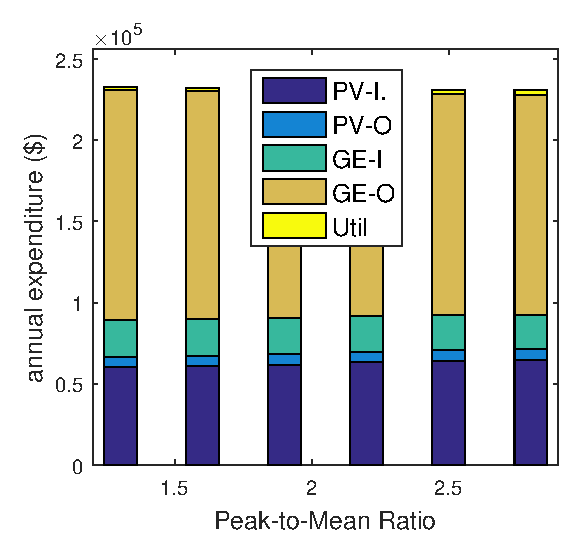
\includegraphics[width=0.32\columnwidth]{figs/cost_PMR}}
			\label{f.cost_PMR}}
		%\subfigure[Payback period]{{\includegraphics[width=0.48\columnwidth]{figs/payback_PMR}}
		\caption{Impacts of interactive workload shapes. The shapes of interactive workload have limited impacts on the capacities and expenditures of GE and PV.}
		\label{f.PMR}
	\end{center}
 \vspace{-0.3cm}
\end{figure}
}

\emph{Shape of interactive workload:} Interactive workload is non-flexible and required to be processed with high responsive speed in data centers. We use the peak-to-mean ratio (PMR) to study the impacts of interactive workload shape. Figure \ref{f.PMR} shows that shape of interactive workload has limited influence on both the capacities and expenditures of data centers. In particular, the capacity of PV and the peak grid power consumption slightly increase as the PMR increases. On the other hand, the data center slightly reduces GE when it has more PV power generation. As the capacities of PV and GE do not vary much, the breakdown expenditures are almost the same when varying the PMRs in Figure {\ref{f.cost_PMR}}.

\hideit{
\begin{figure}[!ht]
%matlab: TCO_grid_payback_ratio.m
\begin{center}
	\subfigure[Capacity]{{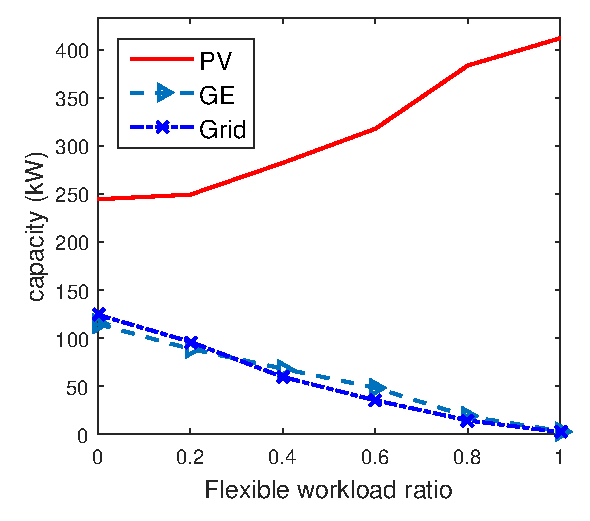
\includegraphics[width=0.32\columnwidth]{figs/capacity_batch}}
		\label{f.capacity_batch}}
	\subfigure[Cost]{{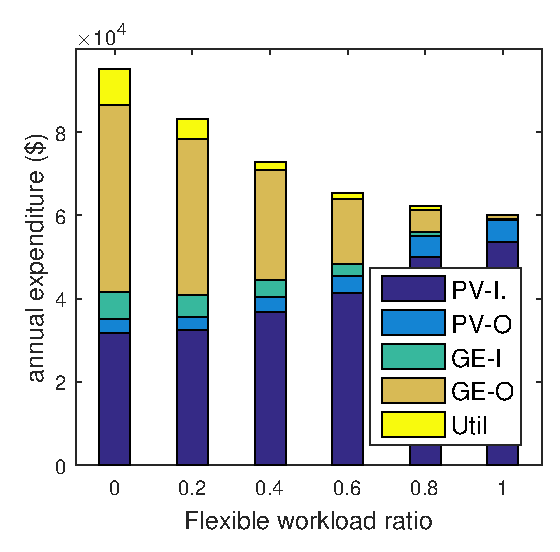
\includegraphics[width=0.32\columnwidth]{figs/cost_batch}}
		\label{f.cost_batch}}
	%\subfigure[Payback period]{{\includegraphics[width=0.48\columnwidth]{figs/payback_batch}}
	%\label{f.payback_batch}}
	\caption{Impacts of flexible workload ratios. The ratio can significantly reduces the total expenditure and change the capacity structure of the data center.}
	\label{f.batch_ratio}
\end{center}
\end{figure}
}
\emph{Ratio of flexible workload} is the ratio of batch jobs to the IT workload demand. The higher ratio of flexible workload means the more flexibility data centers have in power demand management. In particular, Figure~\ref{f.capacity_batch} highlight that the data center is more aggressive in using renewable energy as the ratio of flexible workload increases. It shows that the flexible workloads can promote the use of renewable sources. Especially, when workloads are totally flexible, there is no need to use GE and grid power as the workloads can be scheduled to totally follow PV generation. Figure~\ref{f.cost_batch} shows that the flexible workloads can significantly reduce the total expenditure, e.g., 28\% reduction of the total cost.

\textbf{\textit{Key insights}}: (i) The shape of interactive workload does not affect much on the capacity planning and operational management of data centers. (ii) The flexible workloads promote the use of renewable energy and significantly reduces the total cost.